\documentclass[10pt]{beamer}
\usepackage{graphicx}
\usepackage{adjustbox}
\usepackage[sfdefault]{FiraSans}


\usetheme{metropolis}
\usecolortheme{seagull}  % You can choose from various color themes provided by metropolis


\title[Introduction to Agile Software Development]{
  Introduction to Agile Software Development \\
  \vspace{1cm}
    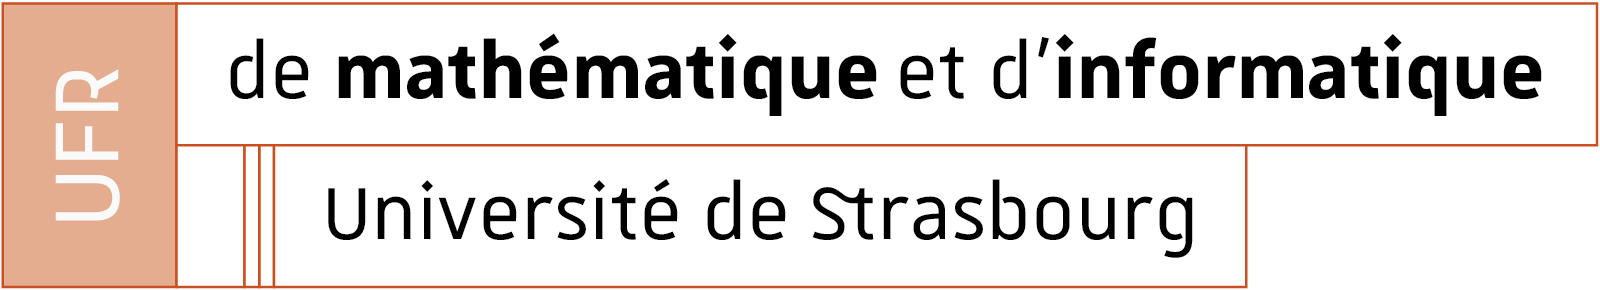
\includegraphics[width=0.6\pdfpagewidth]{images/logo_Uni.png}}

\author[SuperAgile]{Carpi Lapi, Regardin, Senger, Sengler}
\date[February 7, 2024]{February 7, 2024}

\begin{document}

\frame{\titlepage}

\begin{frame}{What is Agile methodology?}
The Agile methodology is a project management approach that involves:
\begin{itemize}
    \item breaking the project into phases
    \item emphasizes continuous collaboration and improvement \\
    \vspace{1cm}
\end{itemize}

Teams follow a cycle of: 
\begin{itemize}
    \item planning
    \item executing
    \item evaluating
\end{itemize}

\end{frame}

% PA %%%%%%%%%%%%%%%%%%%%%%%%%%%%%%%%%%%%%%%%%%%%%%%%%%%%%%%%%%%%%%%%%%%%%%%%%%
\begin{frame}{Agile vs Waterfall}
  \vspace{0.5cm}
  \adjincludegraphics[height=6cm,trim={0 5cm 0 0},clip]{images/agileWater.png}
\end{frame}

\begin{frame}{Agile vs Waterfall}
  \vspace{0.5cm}
  \begin{columns}[T]

    \begin{column}{0.5\textwidth}
      \vspace{2cm}
      \begin{itemize}
        \item<2-> Emphasizes detailed upfront \textbf{planning}
        \item<3-> Progress is measured by meeting project \textbf{milestones}
        \item<4-> Rigidity can lead to \textbf{difficulties in responding to changes}
        \item<5-> Suitable for projects with \textbf{well-defined requirements}
      \end{itemize}
    \end{column}

    \begin{column}{0.5\textwidth}
      \adjincludegraphics[height=14cm,trim={7cm 0 0 9cm},clip]{images/waterfall2.png}
    \end{column}

  \end{columns}
\end{frame}

\begin{frame}{Agile vs Waterfall}
  \vspace{2cm}
  \begin{columns}[T]

    \begin{column}{0.5\textwidth}
      \adjincludegraphics[height=13cm,trim={8cm 0 0 14cm},clip]{images/agile2.png}
    \end{column}

    \begin{column}{0.5\textwidth}
      \begin{itemize}
        \item<2-> \textbf{Iterative} and incremental development 
        \item<3-> Customer \textbf{feedback} is incorporated throughout the process
        \item<4-> Embraces \textbf{flexibility} and customer collaboration
        \item<5-> \textbf{Adaptive approach }to changing requirements
      \end{itemize}
    \end{column}

  \end{columns}
\end{frame}
%%%%%%%%%%%%%%%%%%%%%%%%%%%%%%%%%%%%%%%%%%%%%%%%%%%%%%%%%%%%%%%%%%%%%%%%%%%%%%%

\begin{frame}{General Agile guideline}
    Marie
\end{frame}

\begin{frame}{The Agile Timeline}
    Antoine
\end{frame}

\begin{frame}{Pros and Cons of the Agile Method}
    Antoine
\end{frame}

\begin{frame}{Conclusion}

  Remain flexible, stay agile !
  
\end{frame}

\begin{frame}{References}
  \begin{itemize}
    \item https://www.youtube.com/watch?v=goJu-DFGJ0o
    \item https://www.youtube.com/watch?v=1evfn3qTYGM
    \item https://project-management.com/agile-project-management/
  \end{itemize}
\end{frame}

\end{document}
